\documentclass{TIJMUjiaoanSY}
\pagestyle{empty}


\begin{document}


%课程名称
\kecheng{Linux系统概论}
%实验名称
\shiyan{实验3\ Linux命令行界面的基本操作}
%教师姓名
\jiaoshi{伊现富}
%职称
\zhicheng{讲师}
%教学日期(格式:XXXX年XX月XX日XX时-XX时)
\riqi{2018年5月21日13:30-15:30}
%授课对象(格式:XXX系XXXX年级XX班(硕/本/专科))
\duixiang{生物医学工程学院2016级生信班(本)}
%实验人数
\renshu{28}
%实验类型
\leixing{验证型}
%实验分组
\fenzu{一人一机}
%学时数
\xueshi{2}
%教材版本
\jiaocai{Linux系统概论上机指南(自编教材)}


%教案首页
\firstHeader
\maketitle
\thispagestyle{empty}

\mudi{
\begin{itemize}
  \item 了解使用命令挂载和卸载移动存储介质的方法。
  \item 掌握图形界面下使用shell命令的方法。
  \item 掌握字符界面下使用shell命令的方法。
  \item 掌握ls、cd等常用shell命令的使用。
  \item 掌握软、硬链接的使用方法与异同。
\end{itemize}
}

\fenpei{
\begin{itemize}
  \item (10')Linux用户界面:介绍Linux的两种用户界面——GUI和CLI,并对它们进行比较。
  \item (10')Linux字符界面:介绍进入Linux字符界面的四种方法。
  \item (80')实验操作:以CentOS发行版为例,练习进入字符界面的方法、常用shell命令的使用,比较软链接和硬链接,学习挂载和卸载移动存储介质的命令。
\end{itemize}
}

\cailiao{
\begin{itemize}
  \item 主要仪器:一台安装有CentOS的计算机。
\end{itemize}
}

\zhongdian{
\begin{itemize}
  \item 重点难点:进入字符界面的方法,软链接和硬链接的异同。
  \item 解决策略:通过演示进行学习,通过练习熟练掌握。
\end{itemize}
}

\sikao{
\begin{itemize}
  \item 比较GUI和CLI这两种Linux的用户界面。
  \item 总结进入Linux字符界面的方法。
  \item 总结常用的shell命令及其选项。
  \item 比较软链接和硬链接的异同。
  \item 总结挂载和卸载移动存储介质的命令。
\end{itemize}
}

\cankao{
\begin{itemize}
  \item Linux基础及应用习题解析与实验指导(第二版),谢蓉\ 编著。中国铁道出版社,2014。
\end{itemize}
}

\firstTail


%教案续页
\newpage
\otherHeader

\noindent
\begin{enumerate}
  \item Linux用户界面(10分钟)
    \begin{enumerate}
      \item 两种用户界面
	\begin{itemize}
	  \item 图形用户界面(Graphical User Interface,GUI):指采用图形方式显示的计算机操作用户界面。
	  \item 命令行界面(Command Line Interface,CLI):图形用户界面得到普及之前使用最为广泛的用户界面,它通常不支持鼠标,用户通过键盘输入指令,计算机接收到指令后,予以执行。
	\end{itemize}
      \item GUI vs. CLI\\
	%\vspace*{-10pt}
	\textcolor{red}{Graphical user interfaces make easy tasks easier, while command line interfaces make difficult tasks possible.}
	\begin{itemize}
\parpic[fr]{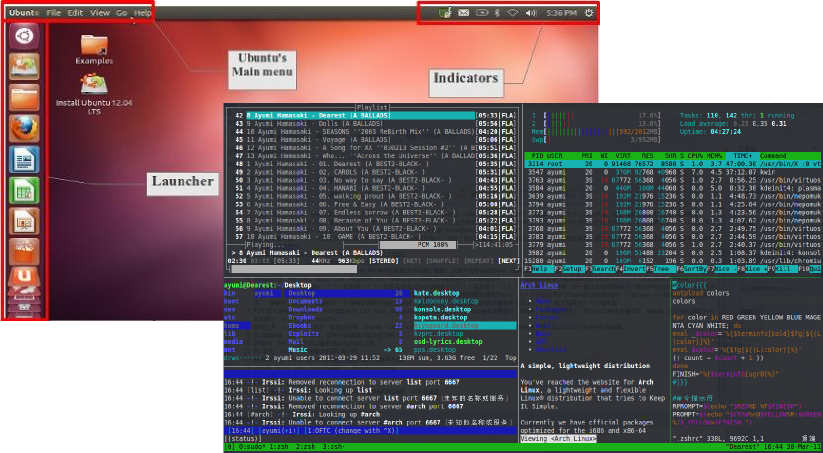
\includegraphics[width=9cm]{c1_gui_cli.png}}
	  \item GUI在视觉上用户更易于接受
	  \item GUI下用户操作简单而且直观
	  \item GUI不能完成所有的操作任务
	  \item GUI的变异性比较大
	  \item CLI占用资源少,启动迅速
	  \item CLI中的操作更加高效
	  \item CLI可完成操作系统所有的工作
	  \item CLI具有高度的相似性
	\end{itemize}
    \end{enumerate}
  \item Linux字符界面(10分钟)
    \begin{enumerate}
      \item 远程登录:ssh \textcolor{gray}{USER@}HOST
      \item 开机直接进入
      \item 虚拟终端:Ctrl + Alt + F[1-6]/F[2-7]\\
	Linux系统都有虚拟终端。虚拟终端为用户提供多个互不干扰、独立工作的工作界面,并且在不同的工作界面可用不同的用户身份登录。虽然用户只面对一个显示器,但可以切换到多个虚拟终端,好像在使用多个显示器。
      \item 终端模拟器:借助于桌面环境下的终端工具使用shell命令
    \end{enumerate}
  \item 实验操作(75分钟)
    \begin{enumerate}
      \item 终端模拟器中的shell命令操作
	\begin{itemize}
	  \item 使用终端模拟器:进入图形界面后,打开“Terminal/终端”
	  \item shell命令练习:date,su,cal,man,cd,ls,……\textcolor{red}{(练习常用选项)}
	\end{itemize}
      \item 虚拟终端中的shell命令操作
	\begin{itemize}
	  \item 进入虚拟终端:进入图形界面后,按Ctrl + Alt + F2切换到虚拟终端,输入用户名和密码
	  \item shell命令练习:pwd,cat,wc,ls,more,head,clear,……\textcolor{red}{(练习常用选项)}
	\end{itemize}
      \item 软链接和硬链接
	\begin{itemize}
	  \item 创建源文件\textcolor{red}{(主要命令:cd,touch,ls -l)}
	  \item 创建链接\textcolor{red}{(主要命令:ln,ln -s,ls -i)}
	  \item 源文件对链接的影响\textcolor{red}{(主要命令:cat,ls -i,rm)}
	  \item 链接对源文件的影响\textcolor{red}{(主要命令:echo,cat,ls -i,rm)}
	\end{itemize}
      \item 挂载和卸载移动存储介质
	\begin{itemize}
	  \item 挂载卸载光盘\textcolor{red}{(主要命令:ls,mount,cp,umount)}
	  \item 挂载卸载U盘\textcolor{red}{(主要命令:mount,ls,df,cp,umount)}
	\end{itemize}
      \item 常见文件与文件夹操作的命令实现
	\begin{itemize}
	  \item 总结图形界面下文件和文件夹的常见操作\textcolor{red}{(如:新建、删除、重命名、移动等)}
	  \item 在字符界面中用命令实现常见操作
	\end{itemize}
    \end{enumerate}
\end{enumerate}


\otherTail


\end{document}

